The core public API\footnote{Application Programming Interface} of \CodeName will be explained, demonstrated and documented in the following chapter. The routines defined, provides facilities to develop powerful and useful extensions and applications, through the minimal but adequate interface. Two examples of extensions empowered by the public \CodeName API are explained subsequently in part \ref{prt:extensions} and are demonstrations of the strength and confirms that all the building blocks needed are available.
\newline

The protocol exposes a vast amount of various \texttt{get}-methods to retrieve useful information regarding the datasets such as metadata, in addition to the routines explained in this chapter.

\section{General}
The formalities which are consistent throughout all of the routines are examined and described in this section.

The API is implemented in Python\cite{PagePython}, which is a high-productivity rather than high-performance programming language that have caught much attention and gained popularity in the high performance and research communities where the utilization thus has increased. The reason for the increased acceptance is because the language easily is extended by open source libraries written in other traditional high-performance languages like Fortran or C++, with a corresponding bridge such as Cython\cite{PageCPython} for C/C++. 
\newline

These types of bridges are are usually an optimising static compilers for Python that simplifies, and minimizes the hard work in the cross language integration. Examples of such library is the de-facto standard in scientific programming, NumPy \cite{PageNumpy} \cite{oliphant2006guide} that is implemented using Cython and Bohrium \cite{PageBohrium} \cite{kristensen2013bohrium} which is a runtime environment for efficiently executing vectorized code on a range of different hardware platforms\footnote{Such as CPU and GPU}.

\begin{quotation}
Python as the main programming language was chosen over others such as C++ and Java based primarily on its high-productivity and thus an appropriate prototype environment in addition to the integration abilities described above.
\end{quotation}

All communication in \CodeName between nodes and the public API is implemented using a Pyro4\cite{PagePyro4}, a remote procedure call library for Python that facilitates communication across the network by minimizing the workload. The library was chosen due to simplicity and precedence with regards to the project scope, but as mentioned in section \ref{sec:communication} there were other alternatives, which in a final solution potentially would increase performance.
\newline

The API seeks to implement a classic CRUD (Create, Read, Update and Delete) pattern with well-known slightly modifications, such as \textit{retrieve} instead of read in terms of the \texttt{get}-methods discussed and an extra \textit{append} functionality to attach data to the dataset.

\section{Create} \label{sec:api-create}
\CodeName provides a dynamic create API call for initializing new empty\footnote{With no data attached} datasets from a required unique name, a required Python class name and package reference like \texttt{example.data.MySpecialDataset} and an optional dictionary of specific extended user and dataset defined metadata attributes, apart from the private configuration \CodeName defined ones.
\newline

The anonymous unique identifier of a dataset is calculated by a hash function\footnote{A mapping function used to represent arbitrary sized data in a fixed space.} and is limited to the key-space size defined in the system configurations, described in details in section \ref{sec:configuration}, to find the responsible root node index (primary replica), which appended to the metadata of the dataset:
\begin{equation}
	\texttt{hash}:name \texttt{ mod } \texttt{\#}keyspace
\end{equation}

The concatenated package and class name are internally transformed to \CodeName \texttt{OperationContext} closure byte stream by compressing\footnote{Using the \texttt{marshall} \cite{PageMarshall} library which by \cite{Brody2015} is approximately 50\% faster than the regular \texttt{cPickle}.} it with an associated digest as a cryptographic signature. The closure is the core of operation execution in \CodeName, which will be explained further in details in section \ref{sec:submit}.

\begin{figure}[ht!]
	\centering
	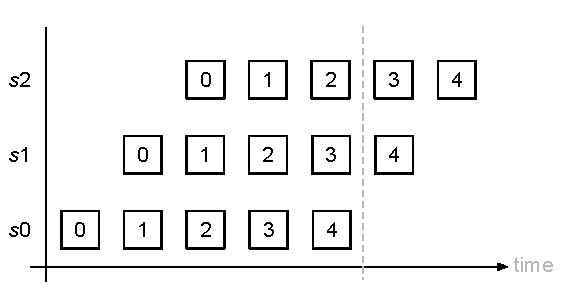
\includegraphics[scale=1.1]{pdf/package-pipeline.pdf}
	\caption{Timing diagram with example of package pipelining \label{fig:package-pipeline}}
\end{figure}	

\section{Append} \label{sec:api-append}
Whenever the frame for a dataset is initialized in \CodeName by the create call, it is possible to append data to it by either one of three ways: \textit{local path}, \textit{url} or \textit{true data}. The unique name that a dataset is initialized with is used whenever any of the other method calls such as \textit{append} or \textit{delete} are utilized. 
\newline

The append call implements the previous described important flow illustrated at Figure \ref{fig:preprocess-nextentry} and thus is the core of succeeding following two objectives (described in details in section \ref{sec:objectives}):

\begin{quotation}
	\textit{Split data such that semantically coherent parts are stored jointly and thus eliminating the data residual problem known from Hadoop.}
\end{quotation}
\noindent
and
\begin{quotation}
	\textit{To store data in arbitrary sized chunks as a consequence of above mentioned.}
\end{quotation}

The responsible dispatcher examined in section \ref{sec:delegation} and depicted at Figure \ref{fig:delegation-framework} is disabled for this particular call only, due to bandwidth rate and latency on transferring new data to a node not responsible for that semantic block of data first before redirected to the right one.

The gateway is for this call capable of determining the responsible server without relaxing excessively on the stateless property, by using the root index added to the metadata in the create-call, to calculate the primary replica index of a specific semantic block:

\vspace*{2mm}
\begin{equation} \label{eq:startindex}
	\Big\lfloor\Big(\texttt{id}:root + \dfrac{\texttt{\#}blocks}{stride}\Big) \texttt{ mod } \texttt{\#}storagenodes\Big\rfloor
\end{equation}

, where the \textit{stride} is a constant specific for each dataset and decided by the distribution strategy, described in section \ref{sec:sofabaseobject}.

\begin{quotation}
	{\sffamily\textbf{NOTE:}} As an aftermath of the abovementioned calculation in equation \ref{eq:startindex}, it is possible henceforth to pick up and append new data to dataset where it left off.
\end{quotation}

\subsubsection*{Package distribution}
Figure \ref{fig:package-pipeline} illustrates a suggestion to an ideal HPC package distribution solution for the append flow implementation, based on the common concept of pipeline computation that Wilkinson \etal describes in \cite{Wilkinson:1998:PPT:289352}. The model is designed to stream fragmented semantic block packages in a pipeline fashion between the gateway and the list of required replicas (as described in section \ref{sec:delegation}) in a priority queue.
\newline

The latency for streaming one package, assuming a network speed of 1 Mb/s and a fragmented package size of 1 MB is:
\begin{equation}
	\dfrac{\texttt{\#}fpackage}{network\text{ }speed} = \dfrac{8\cdot 1024^2 \text{ bits}}{1024^3 \text{ bits/s}} = \dfrac{1}{128} \text{ sec}
\end{equation}

, which with a replication factor of \textit{x} and an assuming total package size of maximum 64 MB (customisable in the system configurations) leads to a replication latency of:
\begin{equation}
	(64 + x - 1) \cdot \dfrac{1}{128} \text{ sec}
\end{equation}

, where the $x - 1$ directly can be derived from Figure \ref{fig:package-pipeline}, with the light gray, dotted line indicates when the first node has finished receiving and transmitting.
\newline

\noindent
Unfortunately, the fragmented package solution explained, requires the communication library applied to support streaming, which Pyro4 doesn't\footnote{Nevertheless, it was chosen based on the criteria and features listed previously.}. The package distribution algorithm implemented in \CodeName is based on the same technology and research as the protocol carried out in the delegation framework, namely the store and forward method. This also means that if the puzzle of replacing the communication library with a more suitable one, it will improve the delegation framework too.
\newline

Current implementation has following latency on sending one 64 MB semantic package and with the same network speed as the previous example:
\vspace*{1mm}
\begin{equation}
	\dfrac{\texttt{\#}package}{network\text{ }speed} = \dfrac{64\cdot 8\cdot 1024^2 \text{ bits}}{1024^3 \text{ bits/s}} = 0.5 \text{ sec}
\end{equation}
\vspace*{2mm}

\noindent
, and thus have a \textit{x} replication latency of:
\begin{equation}
	x \cdot 0.5 \text{ sec}
\end{equation}
 
\section{Update}
Based on the same logic as described in the create call (section \ref{sec:api-create}) but an initialized dataset is a prerequisite before it can be updated.

\section{Delete}
Remove an existing dataset and all associated semantic blocks and replicas, by its 	initiating name.

\section{Submit} \label{sec:submit}
Figure \ref{fig:submit-job} illustrates the bulk synchronous parallel like model implemented in the submit call. The request is forwarded to the responsible replica (described in section \ref{sec:delegation}) before initialization, which if needed is causing a parallel exchange of semantic ghost points (described in section \ref{sec:operation}) on the \textit{n} storage nodes. The interchange happens before the responsible server is initializing the parallel execution of the actual operation, which begins once the $n-1$ storage nodes have reported ready to the root node.
\newline

\begin{figure}
	\centering
	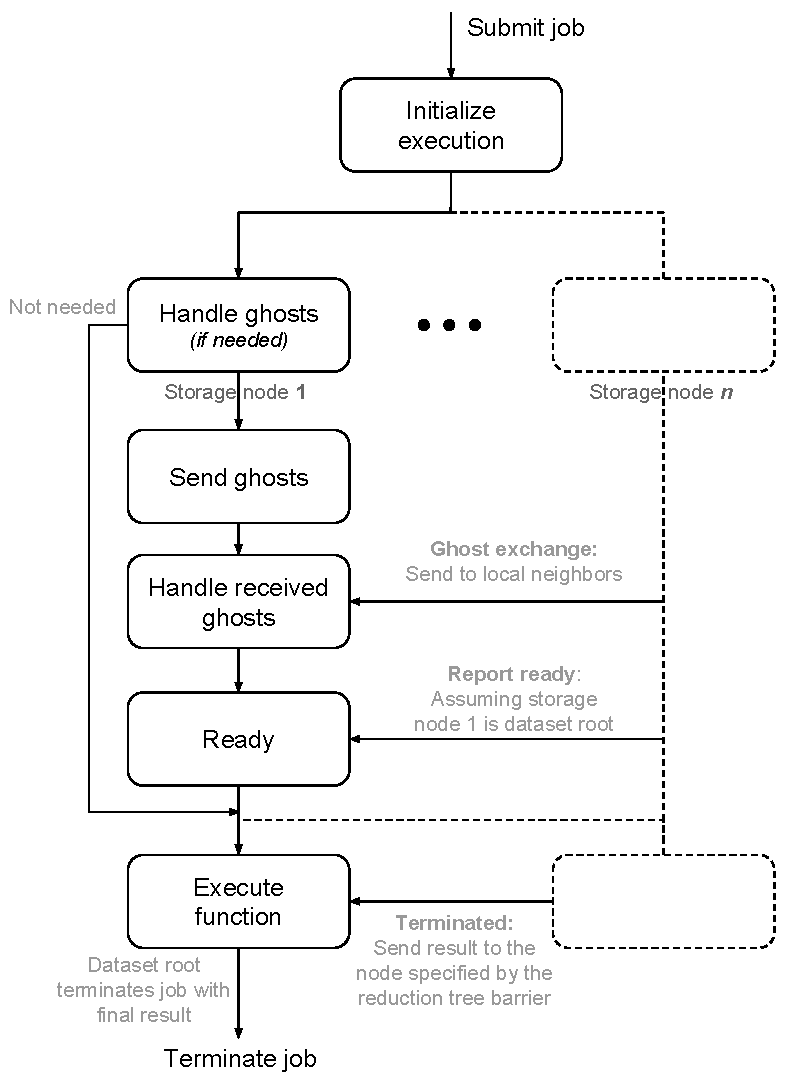
\includegraphics[scale=0.7]{pdf/submit-job.pdf}
	\caption{Flow diagram of the submit API call. \label{fig:submit-job}}
\end{figure}	

\noindent
The reason for the barrier before the execution is to ensure that all storage nodes is in charge of the data required for the calculation, such that no superfluous intercommunication is needed.
\newline

The execution of the operation itself is implemented as a tradeoff between minimizing I/O cost and reducing the load on the root node. The solution is based on the logic of the arrival part of a tree implementation of a barrier as illustrated in the example with 16 storage nodes at Figure \ref{fig:reduction-tree} and explained by Wilkinson \etal in \cite{Wilkinson:1998:PPT:289352}.

A solution particularly well-suited for big data analysis with MapReduce (outlined in definition \ref{def:mapreduce}) as primary data execution model, a statement that is clarified and explained in details with tangible examples in chapter \ref{chp:bdae}.
\newline

The calculation of whom to send to who is based on a multiplication of the \textit{sum of odd numbers}\footnote{$1 + 3 + 5 + \ldots + (2n-1) = n^2$} with respect to the iteration count (the x-axis at the figure). The calculation for any given iteration \textit{i} is as follows:
\begin{equation} \label{eq:reduction}
\underbrace{\dfrac{\texttt{id}:node}{2^{i}}}_{\forall \in \mathbb{N}_0} \texttt{ mod } 2 \equiv 1
\end{equation}
, and will resolve in boolean values that indicate whether the node has to send its result to the closest neighbor on the left-hand side.
\newline

\begin{figure}
	\centering
	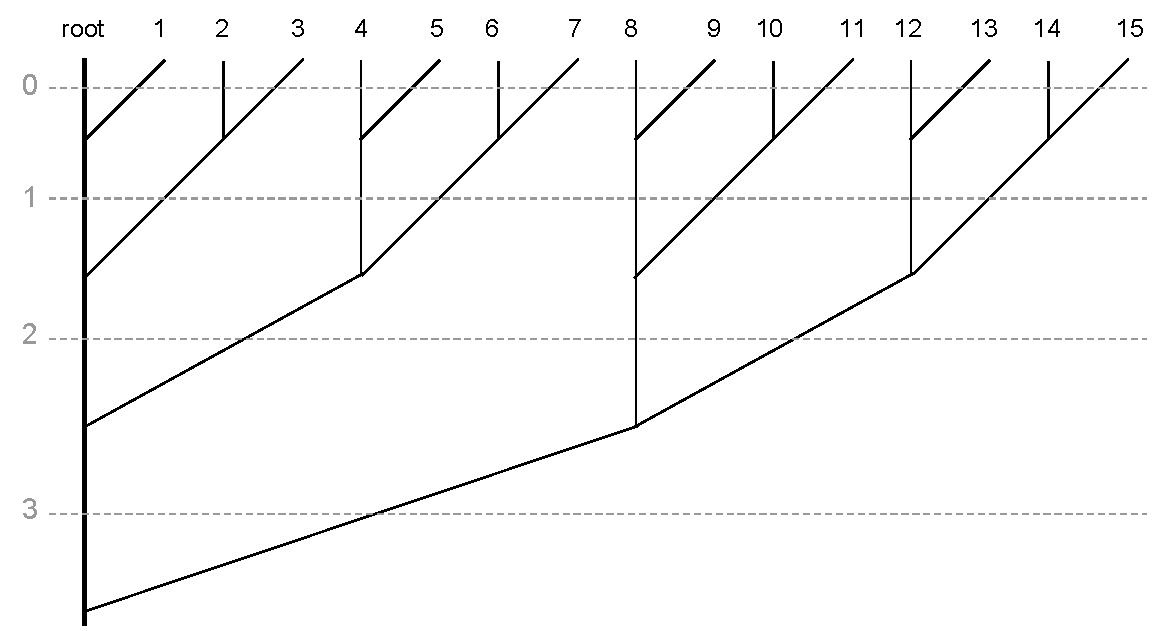
\includegraphics[scale=0.5]{pdf/reduction-tree.pdf}
	\caption[Result reduction calucation example]{Example of a result reduction calucation with 16 storage nodes. \label{fig:reduction-tree}}
\end{figure}	

Each function in the \texttt{OperationContext} is executed in parallel and sequential by the specification from the end-user for the particular procedure. At least one parameter; a block iterator, are required for all functions defined. Hence, the following piece of simple code can be used to iterate over the semantic block content: \texttt{for temp in temperatures: $\ldots$ ;}

\section{Poll}
The poll call is used to check whether the execution of the submitted operation has terminated if the callback of the submit request is vacant.

\section{Documentation}
All the public API calls are documented using Sphinx \cite{PageSphinx} which, using the Python docstring and a \texttt{reStructuredText} markup language layout files is generating intelligent and browsable HTML pages.
